\chapter{Proposed software architecture}
\label{sec:Proposed software architecture}



% \section{Overview}



\section{System architecture choice}
We have chosen to utilise the \textbf{Model-View-Controller} system architecture, separating presentation and interaction from system data. 

\subsubsection{Advantages}
\begin{itemize}
	\item By keeping the visuals separated from the application data, we can achieve very loose coupling, as well as the ability to easily change the same data from many different views, for example via our desktop and web-based clients. \\
	\item If we ever need to change parts of the program, it will be easy to switch out parts of the code.
\end{itemize}


\subsubsection{Disadvantages}
\begin{itemize}
	\item We will most likely have a larger amount of classes than necessary for a project of this scope. \\
	\item The class hierarchy might become messier, as we will need a larger amount of classes for simple tasks.
\end{itemize}


\section{Subsystem decomposition}
We have grouped our classes into subsystems to create a clearer structure of the program. In this section, we will first show an overview of how the subsystems interact, and then a detailed look at the individual subsystems.

%insert subsystem diagrams here



\section{Hardware/software mapping}

\begin{figure}[H]
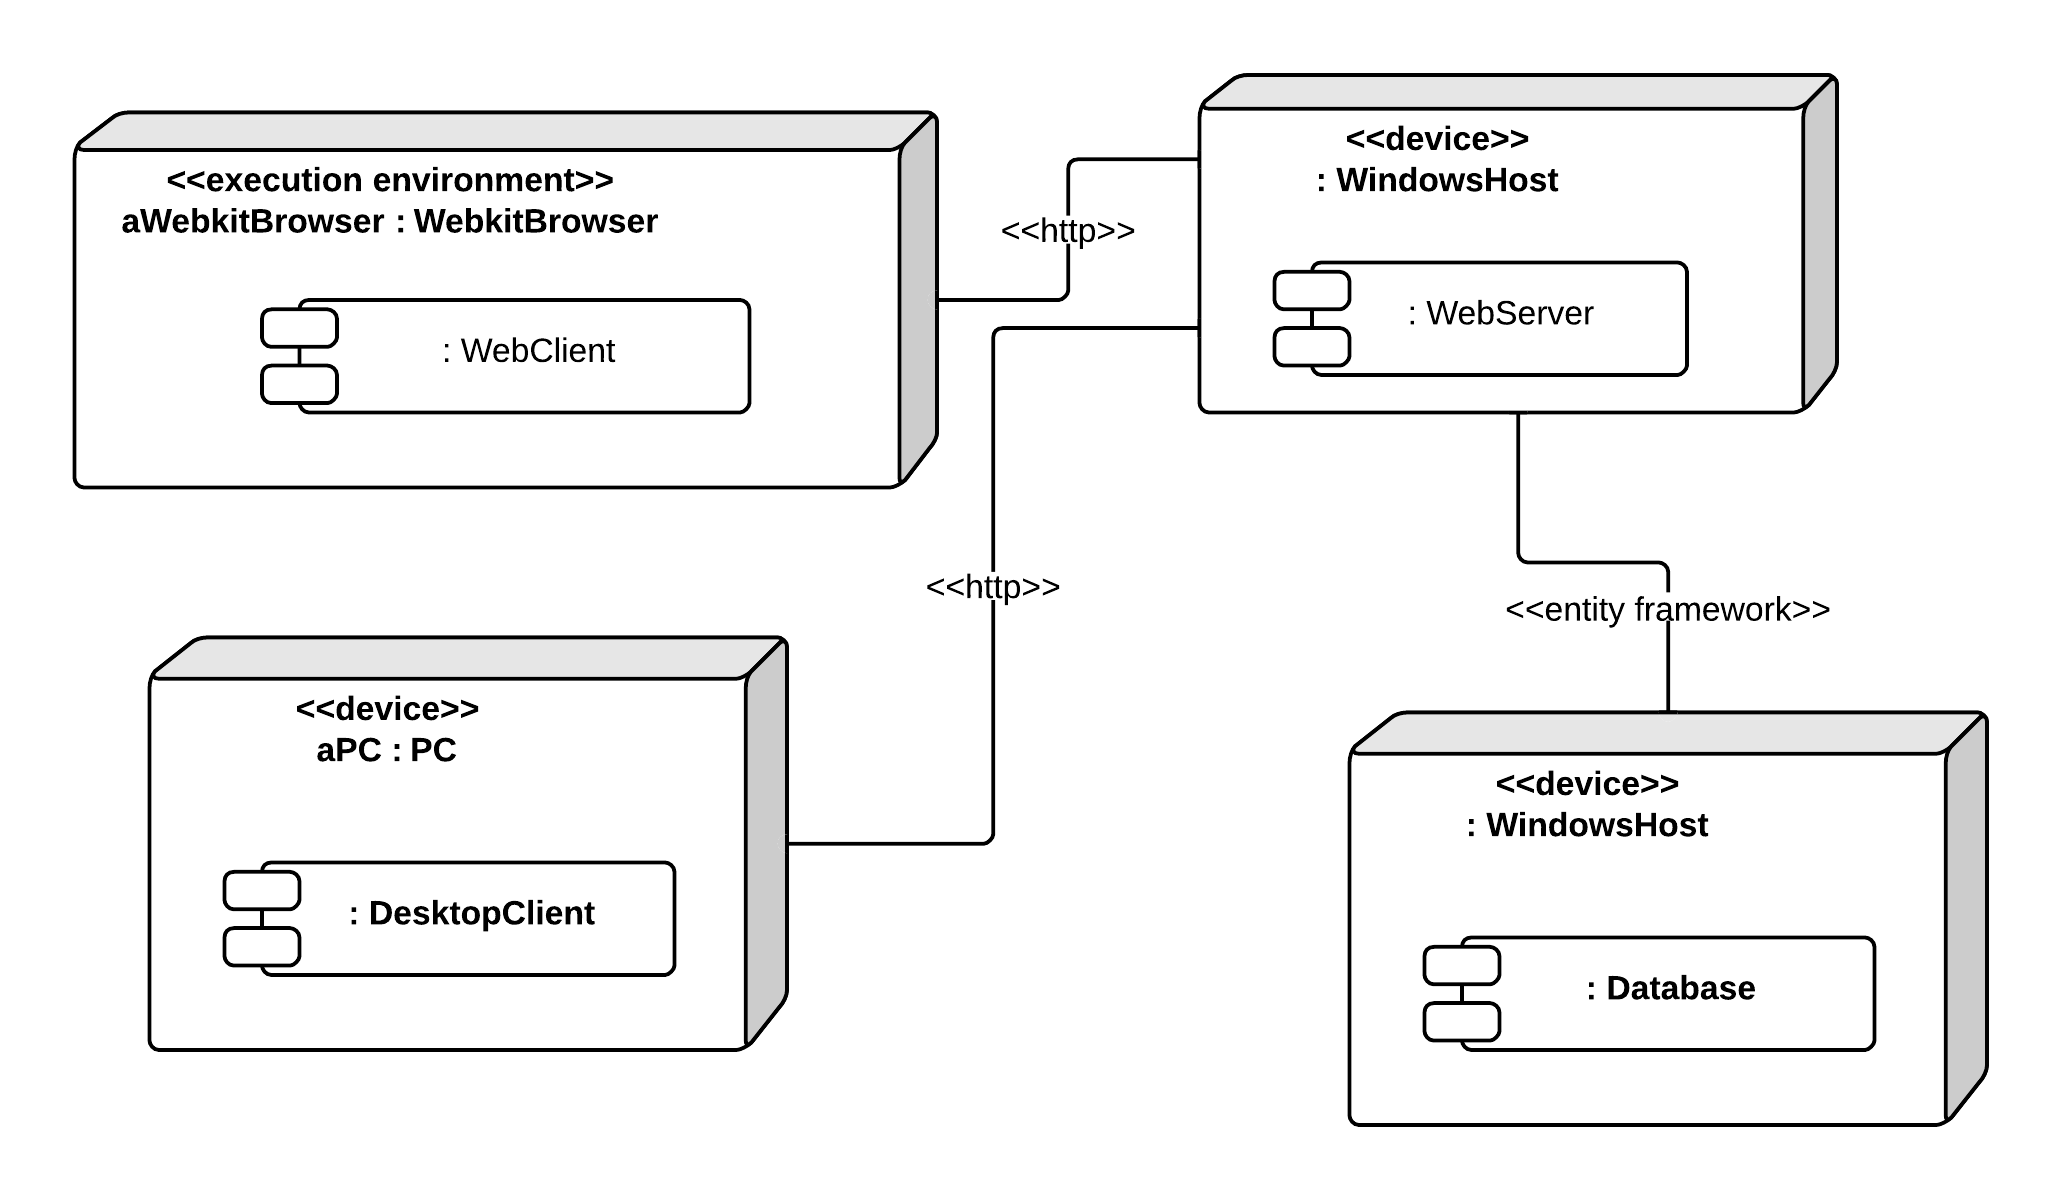
\includegraphics[scale=0.2]{img/SoftwareHardwareMapping.png}
\caption{Software/Hardware Mapping}
\label{fig:SoftwareHardwareMapping}
\end{figure}

\section{Persistent data management}

\subsection{RDBMS mapping}

\section{Access control and security}

\section{Global software control}

\section{Identifying services}

\section{Boundary conditions}

We have indentified the following boundary conditiens, and added them to the list of use cases in the RAD:

\begin{itemize}
	\item Start up and shutdown boundary use cases:
	\begin{itemize}
			\item StartWebServer
			\item ShutdownWebServer
			\item ConfigureWebServer
	\end{itemize}
	\item Exception use cases:
	\begin{itemize}
			\item ServerCrashException
			\item ConnectionLostException
	\end{itemize}
\end{itemize}

\section{Identifying optimization possibilities}